\chapter{Summary of Work Done}

This chapter presents a summary of the work done so far for the project.
Section 2.1 covers the implemented system architecture, while Section 2.2
details the modules implemented for the integrated system.

The source code for the system has been uploaded to GitHub~\cite{gh-magor};
GitHub also serves as the version control and issue management
system~\cite{gh-magor-is} for the project.

\section{System Architecture}

This section outlines the architecture of the implemented transcription system.
 It comprises two independent components --- \textit{modules} and \textit{data} 
--- each resides in its own subfolder within the system. The main system 
executable links these two components together; it executes \textit{procedures},
which are collections of modules in a pipeline, to complete a transcription.

The top level folder structure is as follows:

\begin{lstlisting}
    crawl/
        --raw files--
    data/
        --data files--
    modules/
        --module files--
    system.py               # system executable
    manifest.json           # system manifest
\end{lstlisting}

The whole system would be implemented in Python, using JSON as the manifest
language. The components of the system architecture would be detailed below.

\subsection{Data Folders}

The data used in the system are of two types. The first type is raw data, 
which are unprocessed audio or video files; these files are stored under
\texttt{crawl/}. The second type is processed data, which are stored under
\texttt{data/} in a specialised folder structure:

\begin{lstlisting}
    data/
        file_id/
            raw/
                --the raw file--
            module_1/
                --output for module 1--
            module_2/
                --output for module 2--
            ...
            module_n/
                --output for module n--
            temp/
                module_1/
                    --temporary files for module 1--
                ...
\end{lstlisting}

Under this folder structure, at system startup the system executable would
import the raw file from \texttt{crawl/} into the \texttt{data/file\_id/raw/}
subfolder, with the \texttt{file\_id} being a unique identifier. As a procedure
is being executed, individual module's output files would be stored in the
respective subfolder under \texttt{data/file\_id}, while the module's temporary
files would be stored under \texttt{data/file\_id/temp}.

This structure allows the system to be fully modular; any module would only need
to know its own folder to dump íts output, and practically any operation could
be traced to the module level. Individual modules would be responsible in
implementing this structure.

\subsection{Modules}

All modules in the system are placed under the subfolder \texttt{modules/}
according to the following folder structure:

\begin{lstlisting}
    modules/
        module_id_1/
            setup           # module setup script
            module.py       # module executable
            manifest.json   # module manifest
            --optional module data and executables--
        module_id_2/
            ...
        ...            
\end{lstlisting}

Each module has its own folder; the folder name is a module identifier in
the form of \texttt{module\_name-version}. This allows multiple versions of
a module to co-exist in the system. In each module folder there are three
compulsory components --- a \texttt{setup} script to setup the module and all
its dependencies, a Python executable \texttt{module.py} to call the module,
and a manifest file in JSON format to specify the module details.

The manifest file must conform to this structure:

\begin{lstlisting}
    {
        "name": "module_name",
        "version": "module_version",
        "requires": [],
        "inputs": [],
        "outputs": []
    }
\end{lstlisting}

\texttt{requires}, \texttt{inputs} and \texttt{outputs} are all JSON lists.
\texttt{requires} is a list of (optional) data files and executables required
for the module's functionality; these files should be in place after running
the \texttt{setup} script. \texttt{inputs} and \texttt{outputs} are lists of
subfolders under \texttt{data/file\_id}\footnote{See Section 2.1.1 Data Folders.}
where the module would pull its input files and push its output files, respectively.
In this way, the manifest file serves as a blueprint of the module to the system.
This blueprint would be realised by the \texttt{module.py} executable. Overall,
the three compulsory components work together to ensure each module is self-contained.

\subsection{System Manifest and Executable}

The system manifest specifies system-level properties. It is a JSON file following
this specification:

\begin{lstlisting}
    {
        "procedures": {
            "procedure_id_1": [],
            "procedure_id_2": [],
            ...
        },
        "file_types":{
            "audio": [],
            "video": []
        }
    }
\end{lstlisting}

\texttt{file\_types} would specify which file extensions are accepted by the system;
only raw files of these types would be imported during runtime. The separation of
\texttt{audio} and \texttt{video} types is used for future error-checking.
\texttt{procedures} as mentioned in the beginning of this chapter are pipelines of
modules to perform a certain function. These procedures are specified in the manifest
by unique \texttt{procedure\_ids}; each procedure is a list of \texttt{module\_ids}
\footnote{See Section 2.1.2 Modules.} outlining the order of execution of the modules
on the targeted audio or video file. In this way, the system manifest provides a
blueprint of the whole system to the system executable; it would execute a procedure
according to this flow:

\begin{itemize}
    \item Startup manifest checks --- load all module manifests and system manifest,
    perform error checks and eliminate all ``broken'' modules and procedures
    \item File import --- import the correct files from \texttt{crawl/} into the data
    structure in \texttt{data/}\footnote{See Section 2.1.1 Data Folders.}
    \item Pipeline --- call the modules in the procedure one-by-one in the order
    specified by the system manifest
\end{itemize}

Multiple procedures could be applied to one file, and multiple files could be
processed in one run of the system executable.

\section{Modules and Procedures Implemented}

This section details the modules and procedures implemented so far for the system.
The first part of this section deals with the main task of transcription; the second
part describes the task of keyframe captioning, a related task in video processing,
which demonstrates the extensibility of the system.

The common features across all the implemented modules are:

\begin{itemize}
    \item Robustness --- all modules must check for errors and intermediate state
    completion, and must be able to restart and resume process after any error or
    interruption
    \item Common procedure call --- all modules should be called from the system
    executable in the same manner (the exact manner is
    \texttt{python module.py file\_id})
    \item Logging and error reporting --- all modules should have a common logging
    protocol
\end{itemize}

\subsection{Modules and Procedures for Transcription}

To realize the transcription pipeline in Figure 1.1, three processes must be
modularized: resampling, speaker diarization and transcription. They are detailed
below.

\subsubsection{Resampling}

Audio streams in general comes in many formats with different properties. Before
any processing, the audio stream must be resampled to a common specification; that
specification is usually a format of single-channel PCM (a ``mono'' \texttt{.wav}
file), a sampling rate of 16000 samples per second (16kHz) and a bit rate of 16 bits.

The resampler is implemented using \texttt{FFmpeg}, an open-source, cross-platform
audio and video processing library~\cite{ffmpeg}. The library is well-known and 
well-tested; wrappers around its command-line interface are available for many 
programming languages. For ease of implementation in Python, the Python wrapper
\texttt{FFmpy}~\cite{ffmpy} is used; no additional packages are required.

The module \texttt{resample-1.0} would take an imported audio or video raw file
from \texttt{data/file\_id/raw}, resample it and put the resampled file in
\texttt{data/file\_id/resample}. It is a fairly quick process; no temporary files
are created and successful completion is checked by the presence of the output file.

\subsubsection{Speaker diarization}

After resampling, the audio stream needs to be broken down into smaller segments
for transcription; these segments are usually single-speaker. Audio streams could
be single-speaker or multi-speaker; speaker diarization is performed to produce
single-speaker segments.

The diarizer is implemented using LIUM Speaker Diarization~\cite{lium}, an
open-source package developed by researchers at Laboratoire d'Informatique de
l'Université du Maine. It produces a segmentation file 
(\texttt{.seg})~\cite{lium-seg} which details the start time, end time and
\texttt{speaker\_id} of all identified segments. The source package is in Java;
however there is a convenient command-line interface~\cite{lium} which allows
for a Python wrapper (using the standard Python library module
\texttt{subprocess}).

The module \texttt{diarize-8.4.1} would take a resampled audio stream from
\texttt{data/file\\ \_id/resample}, perform speaker diarization and put the
segmentation file in \texttt{data/file\\ \_id/diarization}. Similar to the
previous module, the process is reasonably fast and successful completion is
checked by the presence of a non-empty output file.

\subsubsection{Transcription}

After successful speaker diarization, the individual segments would be sent
to a transcription engine; the individual transcripts would then be combined
with the timing and speaker information from diarization, to produce the complete
transcription. Two engines are implemented --- the first one based on Google
Cloud Speech API, the second an in-house large vocabulary continuous speech
recognition (LVCSR) system.

\underline{(a) Google Cloud Speech API}

Cloud Speech API~\cite{gcs} is developed by Google, providing the same speech
recognition capabilities powering Google's native applications (such as Voice
Search) to developers. A Python client library (\texttt{google-cloud-speech})
~\cite{gh-gcs} is available which would form the basis of the implemented module.
However to perform speech recognition, one needs to provide a Google API service
account key~\cite{gcs-api-key} and this key is used for usage tracking; the free
tier only allows \$300 of credits to be used in 12 months~\cite{gcs-free}
\footnote{Usage is charged in terms of 15-second blocks; each block is \$0.0025.}.
As such, care must be taken not to exceed the limit; complete checks are heavily
enforced to reduce the number of unnecessary API operations.

The module \texttt{google-1} would take the resampled audio stream from
\texttt{data/file\_id/\\ resample}, split it into individual segments according
to the result from \texttt{data/file\_id/\\diarization}, then sent the segments
to Google Cloud Speech API\@. Intermediate results would be stored in
\texttt{data/file\_id/temp/google}, and the final transcript would be stored in
\texttt{data/file\_id/transcript/google}.

\underline{(b) In-house LVCSR system}

In SLRG, there have been efforts to build a LVCSR system for the English
language~\cite{slrg}. This effort is led by Dr.\ Li Haihua; the system is based
on \texttt{Kaldi}~\cite{kaldi}, an open-source toolkit for speech
recognition written in C++. The system is provided as a black box; the models
and executable are conveniently packaged together. A Python wrapper has been
implemented.

The module \texttt{lvcsr-1701} would take the resampled audio stream from
\texttt{data/file\\ \_id/resample} and the segmentation file from
\texttt{data/file\_id/diarization}, then perform the decoding operation.
Intermediate results would be stored in \texttt{data/file\_id/\\ temp/lvcsr},
and the final transcript would be stored in
\texttt{data/file\_id/transcript/\\lvcsr}.

\subsubsection{Procedures}

As there are two independent engines for transcription, there would be two
procedures applicable for the transcription task. The corresponding system
manifest would be as follows:

\begin{lstlisting}
    {
        "procedures": {
            "google": ["resample-1.0", "diarize-8.4.1", "google-1"],
            "lvcsr": ["resample-1.0", "diarize-8.4.1", "lvcsr-1701"]
        },
        ...
    }
\end{lstlisting}

The two procedures overlap at the first two stages; if both are applied to
a file, for the latter procedure the system executable would skip the
(completed) resampling and diarization and jump straight into transcription.

\subsection{Modules and Procedures for Keyframe Captioning}

In the context of an image, captioning is the process to output a textual
description of said image. This description could contain the objects in the
image as well as their relative positions and relations. An automated captioning
system would be able to recognise such information; coupled with language
understanding, it would be able to produce a human-like summary of the image.

In SLRG, there have been efforts to apply an automated image captioning system
to the specific task of keyframe captioning. A video usually contain many scenes,
each scene identifiable by a keyframe; these keyframes would be extracted out and
captioned in order to derive meaning to a scene, and the results could be indexed
for further use. This work was done by Peter in his final-year project~\cite{peter}
; it is based on Karpathy's \texttt{neuraltalk2} library~\cite{nrtalk2}, which
in turn is bulit upon \texttt{Torch}~\cite{th}, an open-source deep learning
library. Peter's stand-alone system could be converted into a pipeline as follows:

\begin{figure}[h]
\begin{center}
    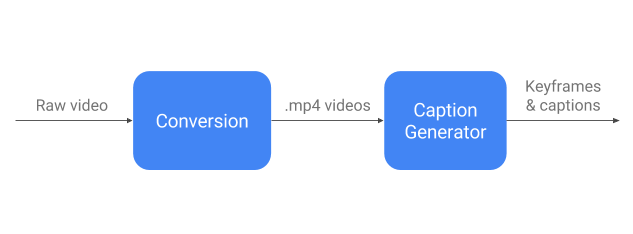
\includegraphics[width=0.9\textwidth]{../images/pipeline_capgen.png}
    \caption{Keyframe captioning processing pipeline}
\end{center}
\end{figure}

Using the same principles applied to the main task of transcription, for keyframe
captioning two components of the pipeline would be modularized: video conversion
and caption generator.

\subsubsection{Video conversion}

Similar to audio streams, video streams come in many different formats. A similar
process to resampling\footnote{See Section 2.2.1 Modules and Procedures for
Transcription.} is employed, which converts different video streams to a common
format --- MPEG Layer 4 video (\texttt{.mp4} files).

The converter is implemented similarly using \texttt{FFmpeg}~\cite{ffmpeg} and the
Python wrapper \texttt{FFmpy}~\cite{ffmpy}. The module \texttt{convert-1.0} would
take a raw video file from \texttt{data/file\_id/\\ raw}, convert it and put the
converted file in \texttt{data/file\_id/convert}. It is a reasonably quick process
as well; no temporary files are created and successful completion is checked by the
presence of the output file.

\subsubsection{Caption generator}

After conversion, the video stream would be extracted for keyframes, and the 
keyframes captioned by \texttt{neuraltalk2}. The module \texttt{capgen-1.0} takes
the converted video file from \texttt{data/file\_id/convert}, then generate
keyframes and their caption into \texttt{data/file\_id/\\ keyframes}. The
temporary files are stored in \texttt{data/file\_id/temp/capgen}.

\subsubsection{Procedure}

The applicable procedure is \texttt{capgen}, and it is specified as follows in
the system manifest:

\begin{lstlisting}
    {
        "procedures": {
            "capgen": ["convert-1.0", "capgen-1.0"]
        },
        ...
    }
\end{lstlisting}

\section{Summary}

In summary, the following body of work has been done to realise the transcription
system:

\begin{table}[h]
\begin{tabularx}{\textwidth}{ll}
    \textbf{Component} & \textbf{Work done} \\
    System architecture & Develop the system architecture \\
    System executable & Develop the Python executable \\
    Module \texttt{resample} & Develop the Python module \\ 
    Module \texttt{diarize} & Develop the Python wrapper
    around external module \\
    Module \texttt{google} & Develop the Python module \\
    Module \texttt{lvcsr} & Modify the existing module to
    fit the system requirements \\
    Module \texttt{convert} & Develop the Python module \\
    Module \texttt{capgen} & Modify the existing module to
    fit the system requirements \\
\end{tabularx}
\end{table}

In addition, the work done has demonstrated, at certain levels, three qualitative
objectives\footnote{See Section 1.2 Objective.} for the system --- Modularity,
Extensibility and Robustness.

The next chapter would focus on the remaining work to be done on the transcription
system.
